\documentclass[12pt,titlepage]{article}
\usepackage[margin=1.25in]{geometry}
\usepackage{graphicx,amsmath,minted}
\usepackage{pgf-umlcd}

%% Variables definition
\newcommand{\vSubject}{Object Oriented Programming}
\newcommand{\vSubtitle}{Class and Object}
\newcommand{\vName}{Dicha Zelianivan Arkana}
\newcommand{\vNIM}{2241720002}
\newcommand{\vClass}{1i}
\newcommand{\vDepartment}{Information Technology}
\newcommand{\vStudyProgram}{D4 Informatics Engineering}

%% [START] Tikz related stuff
\usepackage{tikz}
\usetikzlibrary{svg.path,calc,shapes.geometric,shapes.misc}
\tikzstyle{terminator} = [rectangle, draw, text centered, rounded corners = 1em, minimum height=2em]
\tikzstyle{preparation} = [chamfered rectangle, chamfered rectangle sep=0.75em, draw, text centered, minimum height = 2em]
\tikzstyle{process} = [rectangle, draw, text centered, minimum height=2em]
\tikzstyle{decision} = [diamond, aspect=2, draw, text centered, minimum height=2em]
\tikzstyle{data}=[trapezium, draw, text centered, trapezium left angle=60, trapezium right angle=120, minimum height=2em]
\tikzstyle{connector} = [line width=0.25mm,->]
%% [END] Tikz related stuff

%% [START] Fancy header related stuff
\usepackage{fancyhdr}
\pagestyle{fancy}
\setlength{\headheight}{15pt} % compensate fancyhdr style
\fancyhead{}
\fancyfoot{}
\fancyfoot[L]{\thepage}
\fancyfoot[R]{\textit{\vSubject - \vSubtitle}}
\renewcommand{\footrulewidth}{0.4pt}% default is 0pt, overline for footer
%% [END] Fancy header related stuff

%% [START] Custom tabular command related stuff
\usepackage{tabularx}
\newcommand{\details}[2]{
    #1 & #2  \\
}
%% [END] Custom tabular command related stuff

%% [START] Figure related stuff
\newcommand{\image}[3][1]{
    \begin{figure}[h]
        \centering
        \includegraphics[#1]{#2}
        \caption{#3}
        \label{#3}
    \end{figure}
}
%% [END] Figure related stuff

\begin{document}
\begin{titlepage}
    \centering
    \vfill
    {\bfseries\LARGE
        \vSubject\\
        \vskip0.25cm
        \vSubtitle
    }
    \vfill
    \includegraphics[width=6cm]{images/polinema-logo.png}
    \vfill
    {
        \textbf{Name}\\
        \vName\\
        \vskip0.5cm
        \textbf{NIM}\\
        \vNIM\\
        \vskip0.5cm
        \textbf{Class}\\
        \vClass\\
        \vskip0.5cm
        \textbf{Department}\\
        \vDepartment\\
        \vskip0.5cm
        \textbf{Study Program}\\
        \vStudyProgram
    }
\end{titlepage}

\renewcommand{\umldrawcolor}{black}
\renewcommand{\umlfillcolor}{white}

\section{Practicum}
\subsection{Creating Class Diagram}

Dalam suatu perusahaan salah satu data yang diolah adalah data karyawan. Setiap
karyawan memiliki id, nama, jenis kelamin, jabatan, dan gaji. Setiap karyawan
juga bisa menampilkan data diri pribadi dan melihat gajinya.

\begin{enumerate}
    \item {
        Gambarkan desain class diagram dari studi kasus 1!

        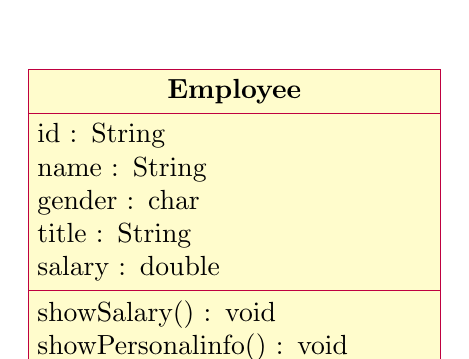
\begin{tikzpicture}
            \begin{class}[text width=5cm]{Employee}{0,0}
                \attribute{id : String}
                \attribute{name : String}
                \attribute{gender : char}
                \attribute{title : String}
                \attribute{salary : double}
                \operation{showSalary() : void}
                \operation{showPersonalinfo() : void}
            \end{class}
        \end{tikzpicture}
    }
    \item {
        Sebutkan Class apa saja yang bisa dibuat dari studi kasus 1!

        \begin{itemize}
            \item \textbf{Employee} - Represents the employee entity
            \item \textbf{Main} - Represents the main program
        \end{itemize}
    }
    \item {
        Sebutkan atribut beserta tipe datanya yang dapat diidentifikasi dari masing-masing class dari studi kasus 1!

        \begin{itemize}
            \item \textbf{id} - String
            \item \textbf{name} - String
            \item \textbf{gender} - char
            \item \textbf{title} - String
            \item \textbf{salary} - double
        \end{itemize}
    }
    \item {
        Sebutkan method-method yang sudah anda buat dari masing-masing class pada studi kasus 1!
    
        \begin{itemize}
            \item \textbf{showSalary()} - Displays the salary of the employee
            \item \textbf{showPersonalinfo()} - Displays the personal information of the employee
        \end{itemize}
    }
\end{enumerate}

\pagebreak

\subsection{Creating and Accessing Class Member}

Perhatikan class diagram dibawah ini. Buatlah program berdasarkan class diagram
tersebut!

\vspace{5mm}

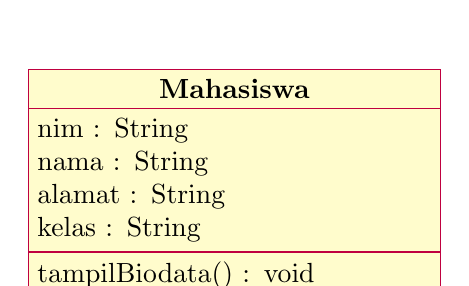
\begin{tikzpicture}
    \begin{class}[text width=5cm]{Mahasiswa}{0,0}
        \attribute{nim : String}
        \attribute{nama : String}
        \attribute{alamat : String}
        \attribute{kelas : String}
        \operation{tampilBiodata() : void}
    \end{class}
\end{tikzpicture}

\begin{itemize}
    \item {
        \textbf{Mahasiswa.java}

        \begin{minted}[autogobble]{java}
            public class Mahasiswa {
                public int nim;
                public String nama;
                public String alamat;
                public String kelas;
            
                public void tampilBiodata() {
                    System.out.println("Nim     : " + nim);
                    System.out.println("Nama    : " + nama);
                    System.out.println("Alamat  : " + alamat);
                    System.out.println("Kelas   : " + kelas);
                }
            }
        \end{minted}
    }
    \item {
        \textbf{TestMahasiswa.java}

        \begin{minted}[autogobble]{java}
            public class TestMahasiswa {
                public static void main(String args[]) {
                    Mahasiswa mhs1 = new Mahasiswa();
                    mhs1.nim = 101;
                    mhs1.nama = "Lestari";
                    mhs1.alamat = "Jl. Vinolia No 1A";
                    mhs1.kelas = "1A";
                    mhs1.tampilBiodata();
                }
            }
        \end{minted}
    }
\end{itemize}

\pagebreak

\begin{enumerate}
    \item {
        Jelaskan pada bagian mana proses pendeklarasian atribut pada program diatas!

        \begin{minted}[autogobble]{java}
            public int nim;
            public String nama;
            public String alamat;
            public String kelas;
        \end{minted}
    }
    \item {
        Jelaskan pada bagian mana proses pendeklarasian method pada program diatas!

        \begin{minted}[autogobble]{java}
            public void tampilBiodata() {
                System.out.println("Nim     : " + nim);
                System.out.println("Nama    : " + nama);
                System.out.println("Alamat  : " + alamat);
                System.out.println("Kelas   : " + kelas);
            }
        \end{minted}
    }
    \item {
        Berapa banyak objek yang di instansiasi pada program diatas!

        There's only one object that was instantiated, which is shown in the code below.

        \begin{minted}[autogobble]{java}
            Mahasiswa mhs1 = new Mahasiswa();
        \end{minted}
    }
    \item {
        Apakah yang sebenarnya dilakukan pada sintaks program \texttt{mhs1.nim = 101} ?

        It assigns the number 101 to the \texttt{nim} attribute of the \texttt{mhs1} object.
    }
    \item {
        Apakah yang sebenarnya dilakukan pada sintaks program \texttt{mhs1.tampilBiodata()} ?

        It calls the \texttt{tampilBiodata()} method of the \texttt{mhs1} object which will
        display the biodata of the object.
    }
    \item {
        Instansiasi 2 objek lagi pada program diatas!

        \begin{minted}[autogobble]{java}
            Mahasiswa mhs2 = new Mahasiswa();
            mhs2.nim = 102;
            mhs2.nama = "Dewi";
            mhs2.alamat = "Jl. Vinolia No 1B";
            mhs2.kelas = "1B";
            mhs2.tampilBiodata();

            Mahasiswa mhs3 = new Mahasiswa();
            mhs3.nim = 103;
            mhs3.nama = "Agus";
            mhs3.alamat = "Jl. Vinolia No 1C";
            mhs3.kelas = "1C";
            mhs3.tampilBiodata();
        \end{minted}
    }
\end{enumerate}

\subsection{Writing method with arguments/parameters and return value}

\begin{itemize}
    \item {
        \textbf{Barang.java}

        \begin{minted}[autogobble]{java}
            public class Barang {
                public String namaBarang;
                public String jenisBarang;
                public int stok;

                public void tampilBarang() {
                    System.out.println("Nama Barang     : " + namaBarang);
                    System.out.println("Jenis Barang    : " + jenisBarang);
                    System.out.println("Stok            : " + stok);
                }

                // method dengan argument dan nilai balik (return value)
                public int tambahStok(int brgMasuk) {
                    int stokBaru = brgMasuk + stok;
                    return stokBaru;
                }
            }
        \end{minted}
    }
    \item {
        \textbf{TestBarang.java}

        \begin{minted}[autogobble]{java}
            public class TestBarang {
                public static void main(String args[]) {
                    Barang brg1 = new Barang();
                    brg1.namaBarang = "Pensil";
                    brg1.jenisBarang = "ATK";
                    brg1.stok = 10;
                    brg1.tampilBarang();
                    // menampilkan dan mengisi argumen untuk menambahkan stok barang
                    System.out.println("Stok Baru adalah " + brg1.tambahStok(20));
                }
            }
        \end{minted}
    }
\end{itemize}

\begin{enumerate}
    \item {
        Apakah fungsi argumen dalam suatu method?

        Arguments are used to pass data to a method.
    }
    \item {
        Ambil kesimpulan tentang kegunaan dari kata kunci return, dan kapan suatu method
        harus memiliki return!

        The \texttt{return} keyword is used to return a value from a method. We'd use it
        if we want to return a value from a method. This is useful to compose methods
        together.
    }
\end{enumerate}

\section{Task}
\subsection{Task 1}
\begin{enumerate}
    \item {
        Suatu toko persewaan video game salah satu yang diolah adalah peminjaman, dimana
        data yang dicatat ketika ada orang yang melakukan peminjaman adalah id, nama
        member, nama game, dan harga yang harus dibayar. Setiap peminjaman bisa
        menampilkan data hasil peminjaman dan harga yang harus dibayar. Buatlah class
        diagram pada studi kasus diatas!

        \begin{itemize}
            \item Harga yang harus dibayar diperoleh dari lama sewa x harga
            \item Diasumsikan 1x transaksi peminjaman game yang dipinjam hanya 1 game saja
        \end{itemize}

        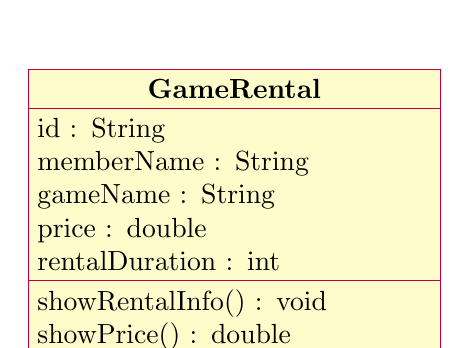
\begin{tikzpicture}
            \begin{class}
                {GameRental}{0,0}
                \attribute{id : String}
                \attribute{memberName : String}
                \attribute{gameName : String}
                \attribute{price : double}
                \attribute{rentalDuration : int}
                \operation{showRentalInfo() : void}
                \operation{showPrice() : double}
            \end{class}
        \end{tikzpicture}
    }
    \item {
        Buatlah program dari class diagram yang sudah anda buat di no 1!

        \begin{minted}[autogobble]{java}
            public class GameRental {
                public String id;
                public String memberName;
                public String gameName;
                public double price;
                public int rentalDuration;

                public void showRentalInfo() {
                    System.out.println("ID          : " + id);
                    System.out.println("Member Name : " + memberName);
                    System.out.println("Game Name   : " + gameName);
                    System.out.println("Price       : " + price);
                    System.out.println("Duration    : " + rentalDuration);
                }

                public double showPrice() {
                    return price * rentalDuration;
                }
            }
        \end{minted}
    }
    \item {
        Buatlah program sesuai dengan class diagram berikut ini:

        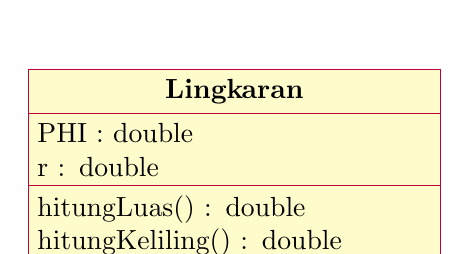
\begin{tikzpicture}
            \begin{class}[text width=5cm]{Lingkaran}{0,0}
                \attribute{PHI : double}
                \attribute{r : double}
                \operation{hitungLuas() : double}
                \operation{hitungKeliling() : double}
            \end{class}
        \end{tikzpicture}

        \begin{minted}[autogobble]{java}
            public class Lingkaran {
                public static final double PHI = 3.14;
                public double r;

                public double hitungLuas() {
                    return PHI * r * r;
                }

                public double hitungKeliling() {
                    return 2 * PHI * r;
                }
            }
        \end{minted}
    }
    \pagebreak
    \item {
        Buatlah program sesuai dengan class diagram berikut ini:

        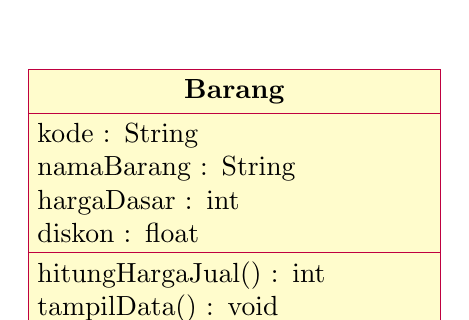
\begin{tikzpicture}
            \begin{class}
                {Barang}{0,0}
               \attribute{kode : String}
                \attribute{namaBarang : String}
                \attribute{hargaDasar : int}
                \attribute{diskon : float}
                \operation{hitungHargaJual() : int}
                \operation{tampilData() : void}
            \end{class}
        \end{tikzpicture}

        Deskripsi / Penjelasan :
        \begin{itemize}
            \item Nilai atribut hargaDasar dalam Rupiah dan atribut diskon dalam \%
            \item {
                Method \texttt{hitungHargaJual()} digunakan untuk menghitung harga jual dengan
                perhitungan berikut ini:

                $$harga jual = harga dasar - (diskon \times harga dasar)$$
            }
            \item {
                Method tampilData() digunakan untuk menampilkan nilai dari kode, namaBarang,
                hargaDasar, diskon dan harga jual
            }
        \end{itemize}

        \begin{minted}[autogobble]{java}
            public class Barang {
                public String kode;
                public String namaBarang;
                public int hargaDasar;
                public float diskon;

                public int hitungHargaJual() {
                    return hargaDasar - (int) (diskon * hargaDasar);
                }

                public void tampilData() {
                    System.out.println("Kode        : " + kode);
                    System.out.println("Nama Barang : " + namaBarang);
                    System.out.println("Harga Dasar : " + hargaDasar);
                    System.out.println("Diskon      : " + diskon);
                }
            }
        \end{minted}
    }
\end{enumerate}

\end{document}

